\documentclass{article}

\usepackage[utf8]{inputenc}
\usepackage[T1]{fontenc}
\usepackage{datetime}
\usepackage{graphicx}
\usepackage{float}
\usepackage{subcaption}

\usepackage{minted}
\usepackage[os=win]{menukeys}
\usepackage{tikz}

\usepackage[english]{babel}
\usepackage{geometry}

\usepackage{adjustbox}
\usepackage{multirow}
\usepackage{hyperref}
\usepackage{titlesec}

\geometry{
	a4paper,
	left=25mm,
	right=25mm,
	top=25mm,
	bottom=25mm,
}

\hypersetup{
	colorlinks=true,
	linkcolor=blue,
	urlcolor=blue,
}

\setcounter{secnumdepth}{4}
\renewcommand{\theparagraph}{\thesubsubsection.\alph{paragraph}}

\addto\captionsenglish{\renewcommand{\contentsname}{Daftar Isi}}
\addto\captionsenglish{\renewcommand{\tablename}{Tabel}}
\addto\captionsenglish{\renewcommand{\figurename}{Gambar}}

\def\mydate{\leavevmode\hbox{\the\year-\twodigits\month-\twodigits\day}}
\def\twodigits#1{\ifnum#1<10 0\fi\the#1}

% this custom commands below will not work if not run on GNU/Linux
\newcommand{\ShowOsVersion}{
	\immediate\write18{\unexpanded{foo=`uname -srom | tr '_' '-'` && echo -n "${foo}" > tmp.txt}}
	\unskip\unskip\input{tmp.txt}\unskip
	\immediate\write18{rm tmp.txt}
}
\newcommand{\ShowTexVersion}{
	\immediate\write18{\unexpanded{foo=`pdflatex -version | head -n1 | cut -d' ' -f1,2` && echo -n "${foo}" > tmp.txt}}
	\unskip\unskip\input{tmp.txt}\unskip
	\immediate\write18{rm tmp.txt}
}

\begin{document}
	\begin{titlepage}
		\centering

		{
			\LARGE
			\bf
			Laporan Kegiatan Uji Mandiri Audiometri Portabel
		}

		\bigskip

		{
			\large
			\bf
			Tim Penelitian Audiometer Portable Elbicare
		}

		\vfill

		\begin{figure}[H]
			\centering
			
\includegraphics[width=250pt,angle=0]{images/elbicare-logo}
		\end{figure}

		\vfill

		\bigskip

		{
			\bf
			Achmadi ST MT dan M. Ammar Asyraf ST MT
		}
	\end{titlepage}

%	\newpage
%
%	\textbf{Tentang Dokumen}\\
%
%	\noindent Dokumen ini ditulis menggunakan {\textbf{\ShowTexVersion}}pada sistem operasi {\textbf{\ShowOsVersion}}yang
%	diupdate terakhir pada tanggal {\mydate} di jam \currenttime.\\
%
%	Kode sumber dokumen ini dapat ditemukan di laman repositori proyek
%	\url{https://github.com/VibrasticLab/pikoakustik2/tree/master/prototrial/dokumen/berita_acara/itb_july2023/test_self}.

	\newpage

	\tableofcontents

	\newpage
	\section{Pendahuluan}

	Dokumen ini adalah rangkuman kegiatan uji mandiri perangkat Audiometri Portabel.

	\subsection{Tujuan Kegiatan}

	Tujuan utama kegiatan ini adalah mendapatkan konversi skala \textbf{loudness} dari nada murni menjadi nilai aktual dalam dB-SPL untuk setiap frekuensi uji.

	\subsection{Waktu dan Tempat}

	Kegiatan ini dilakukan di Ruang Dengung dan Ruang Kedap Gedung Adhiwijogo di Institut Teknologi Bandung pada tanggal 10 Juli 2023.

	\subsection{Alat dan Perlengkapan}

	Alat dan perlengkapan meliputi:

	\begin{itemize}
		\item Sound Level Meter Merek Rion yang telah terkalibrasi.

		\begin{figure}[H]
			\centering
			\begin{subfigure}[]{.35\textwidth}
				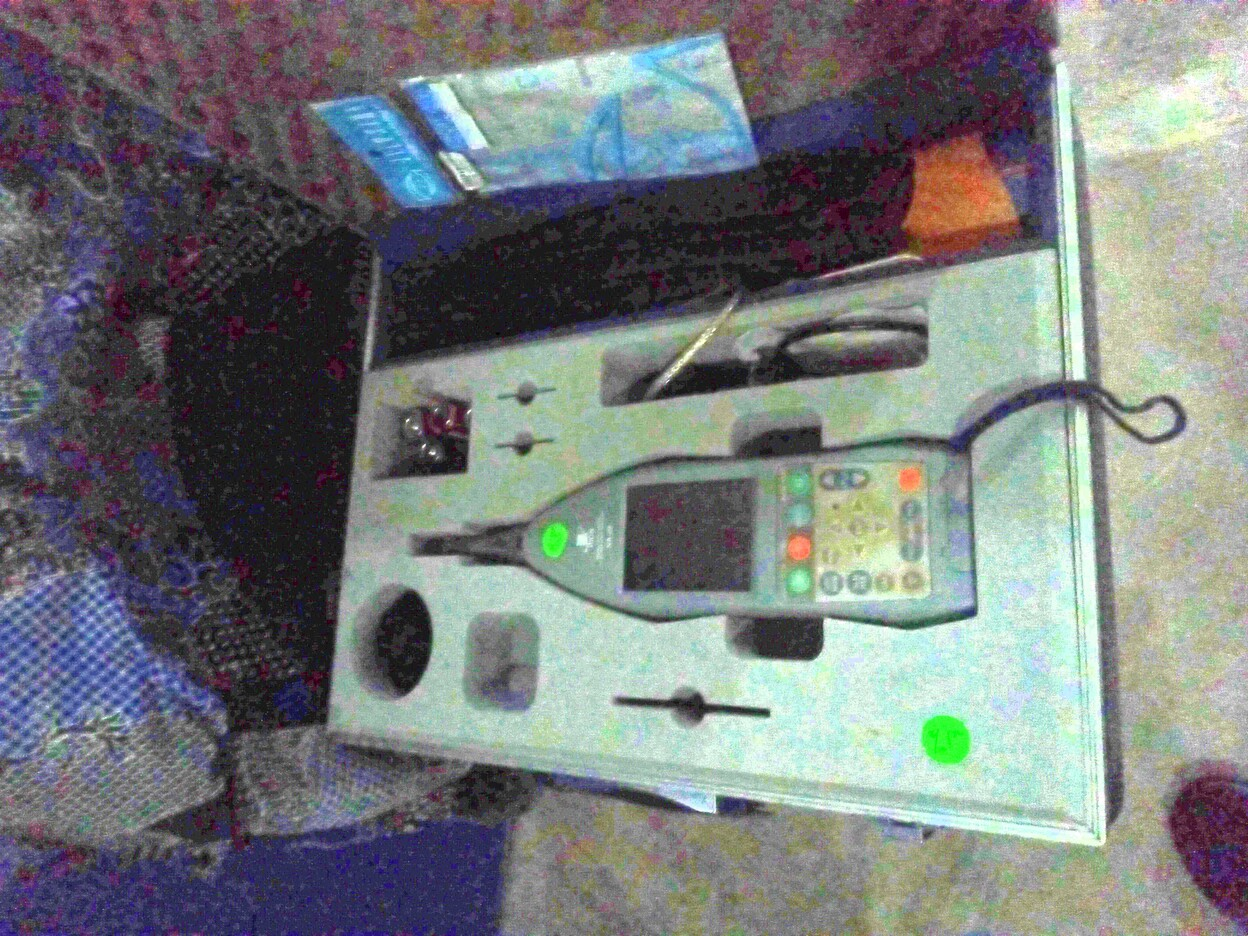
\includegraphics[width=\textwidth]{images/tools_slm_box}
				\caption{SLM RION}
			\end{subfigure}
			\begin{subfigure}[]{.25\textwidth}
				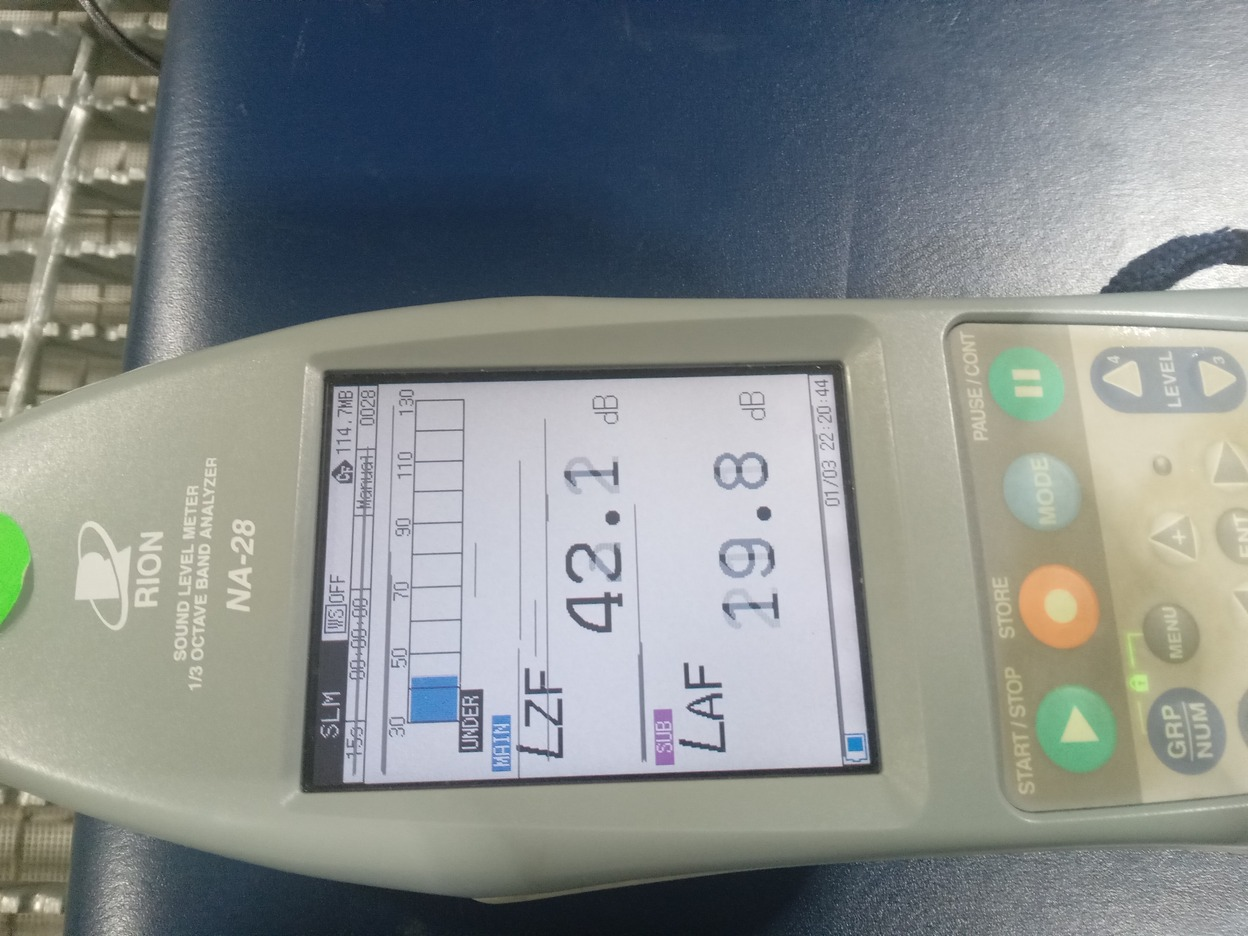
\includegraphics[width=\textwidth]{images/slm_lowest}
				\caption{Noise paling rendah}
			\end{subfigure}
			\caption{Perangkat SLM}
		\end{figure}

		\item Paket Audiometri yang terdiri dari Konsol Audiometri, Headphone JBL T500, dan Kabel USB

		\begin{figure}[H]
			\centering
			\begin{subfigure}[]{.35\textwidth}
				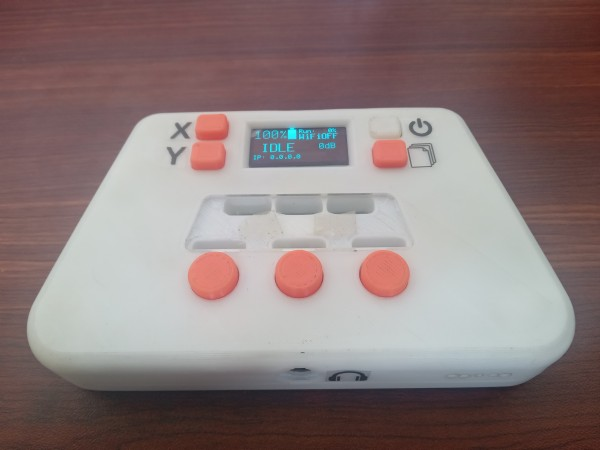
\includegraphics[width=\textwidth]{images/proto}
				\caption{Prototype Konsol}
			\end{subfigure}
			\begin{subfigure}[]{.25\textwidth}
				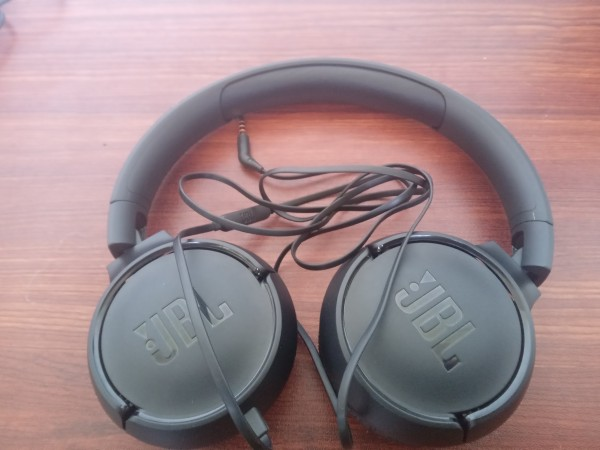
\includegraphics[width=\textwidth]{images/jbl}
				\caption{Headphone JBL}
			\end{subfigure}
			\\
			\begin{subfigure}[]{.25\textwidth}
				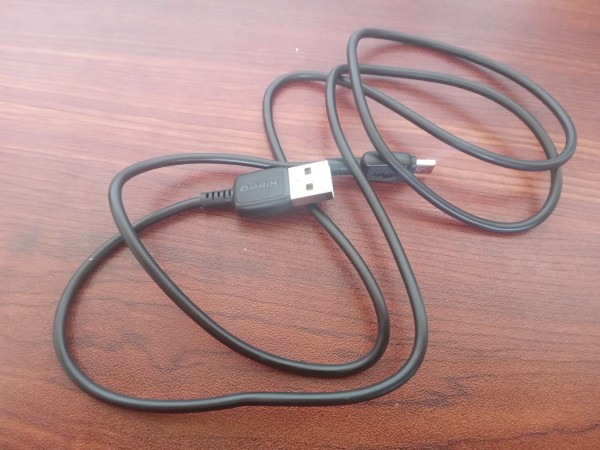
\includegraphics[width=\textwidth]{images/kabel}
				\caption{Kabel USB}
			\end{subfigure}
			\caption{Perangkat Audiometri}
		\end{figure}

		\item Unit Microphone 3DIO dan AudioBox Presonus USB96. Ini adalah unit simulator telinga kedua.
		Berikut laman produk: \href{https://3diosound.com/products/free-space-pro-binaural-microphone}{3DIO}
		dan \href{https://www.frontendaudio.com/presonus-audiobox-usb-96-usb-audio-interface/}{AudioBox USB96}

		\begin{figure}[H]
			\centering
			\begin{subfigure}[]{.40\textwidth}
				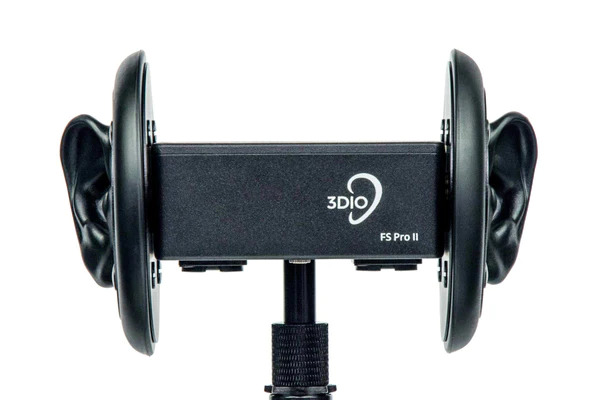
\includegraphics[width=\textwidth]{images/3dio}
				\caption{Microphone 3DIO}
			\end{subfigure}
			\begin{subfigure}[]{.40\textwidth}
				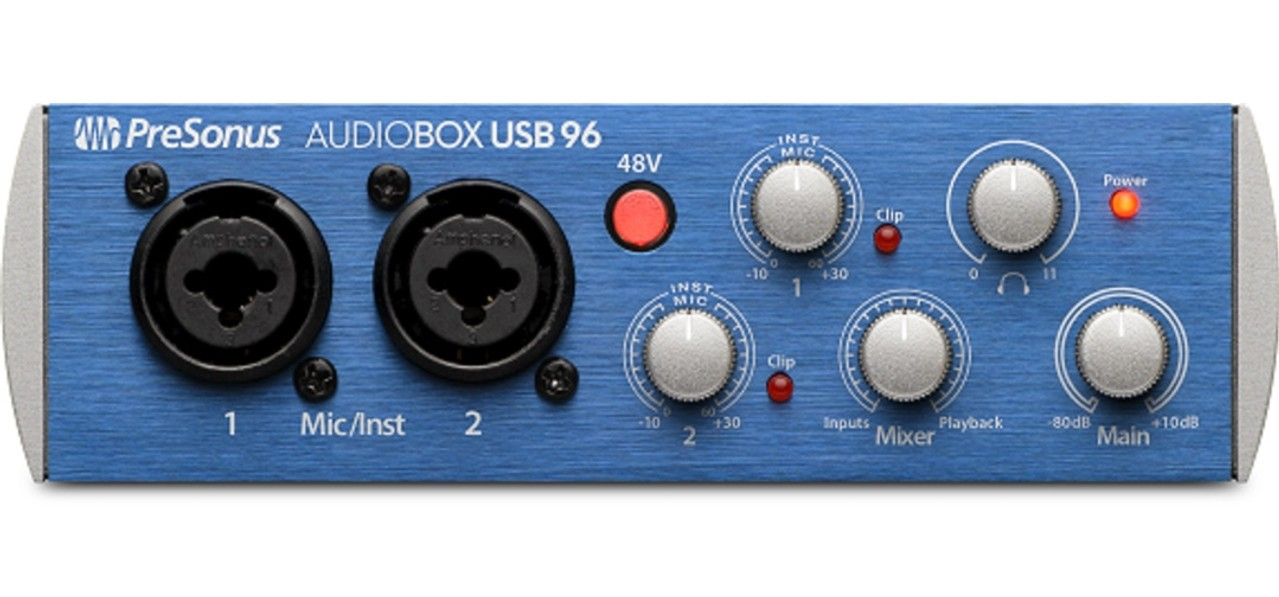
\includegraphics[width=\textwidth]{images/audiobox}
				\caption{Audiobox USB96}
			\end{subfigure}
			\caption{Perangkat 3DIO}
		\end{figure}

%		\item Sebagai pembanding, digunakan perangkat KEMAR dengan metode yang kurang lebih sama.
%		Laman produk: \href{https://www.grasacoustics.com/products/head-torso-simulators-kemar/product/733-45bb}{KEMAR}
%
%		\begin{figure}[H]
%			\centering
%			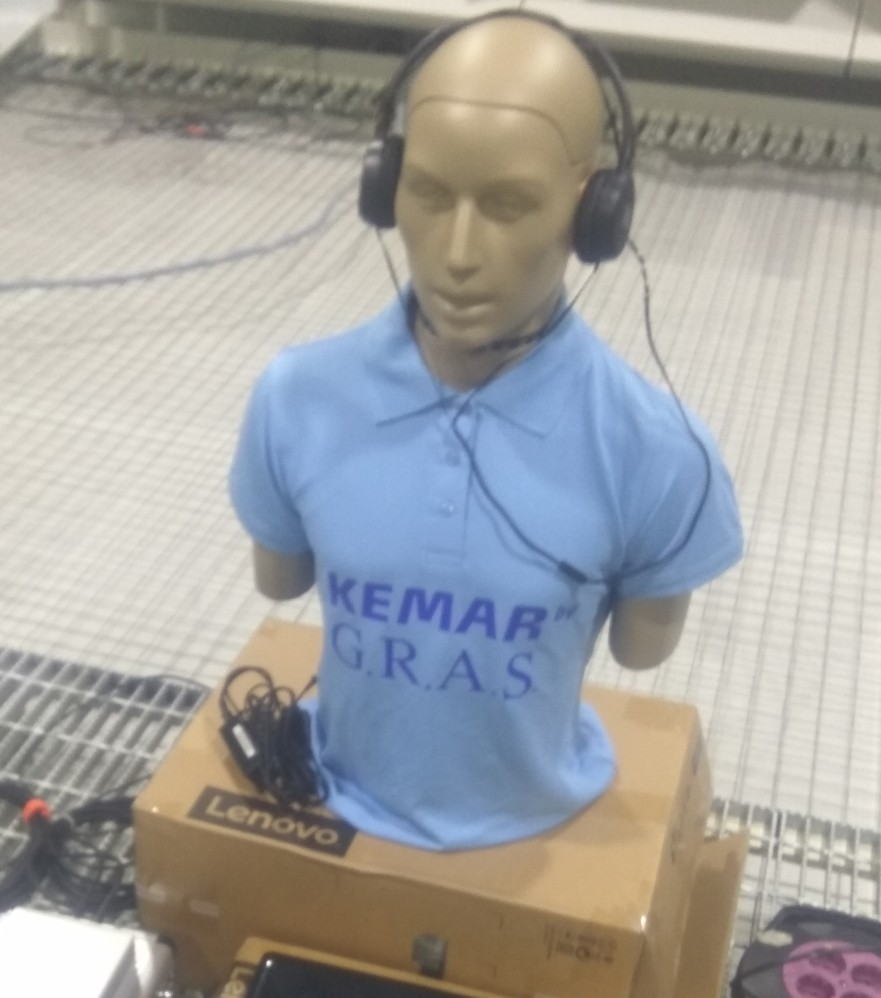
\includegraphics[width=0.35\textwidth,angle=0]{images/kemar}
%			\caption{Perangkat KEMAR}
%		\end{figure}

		\item Perangkat Lunak RealTime Analyzer dari Yoshimasa.
		Berikut laman produk: \href{http://www.ymec.com/products/dssf3e/}{RTA}.

		\begin{figure}[H]
			\centering
			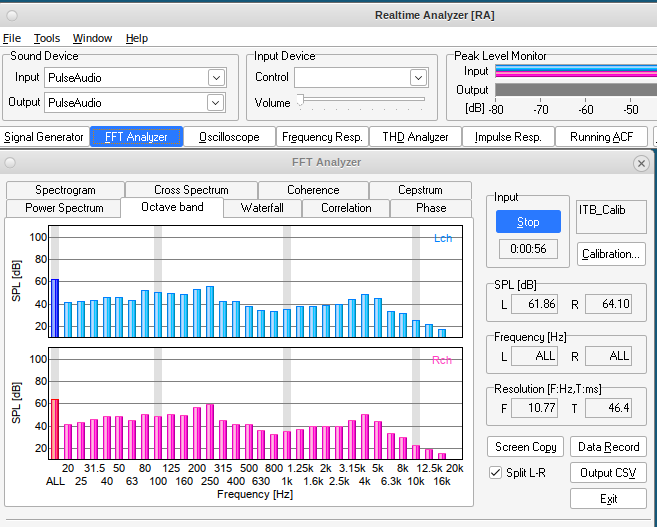
\includegraphics[width=0.75\textwidth,angle=0]{images/rta_fft}
			\caption{Perangkat Lunak RTA}
		\end{figure}

	\end{itemize}

	\newpage

	\section{Setup Pengujian}

	\subsection{Diagram Pengujian}

	Berikut Diagram Pengujian yang disiapkan:

%	\begin{figure}[H]
%		\centering
%		\begin{subfigure}[]{.45\textwidth}
%			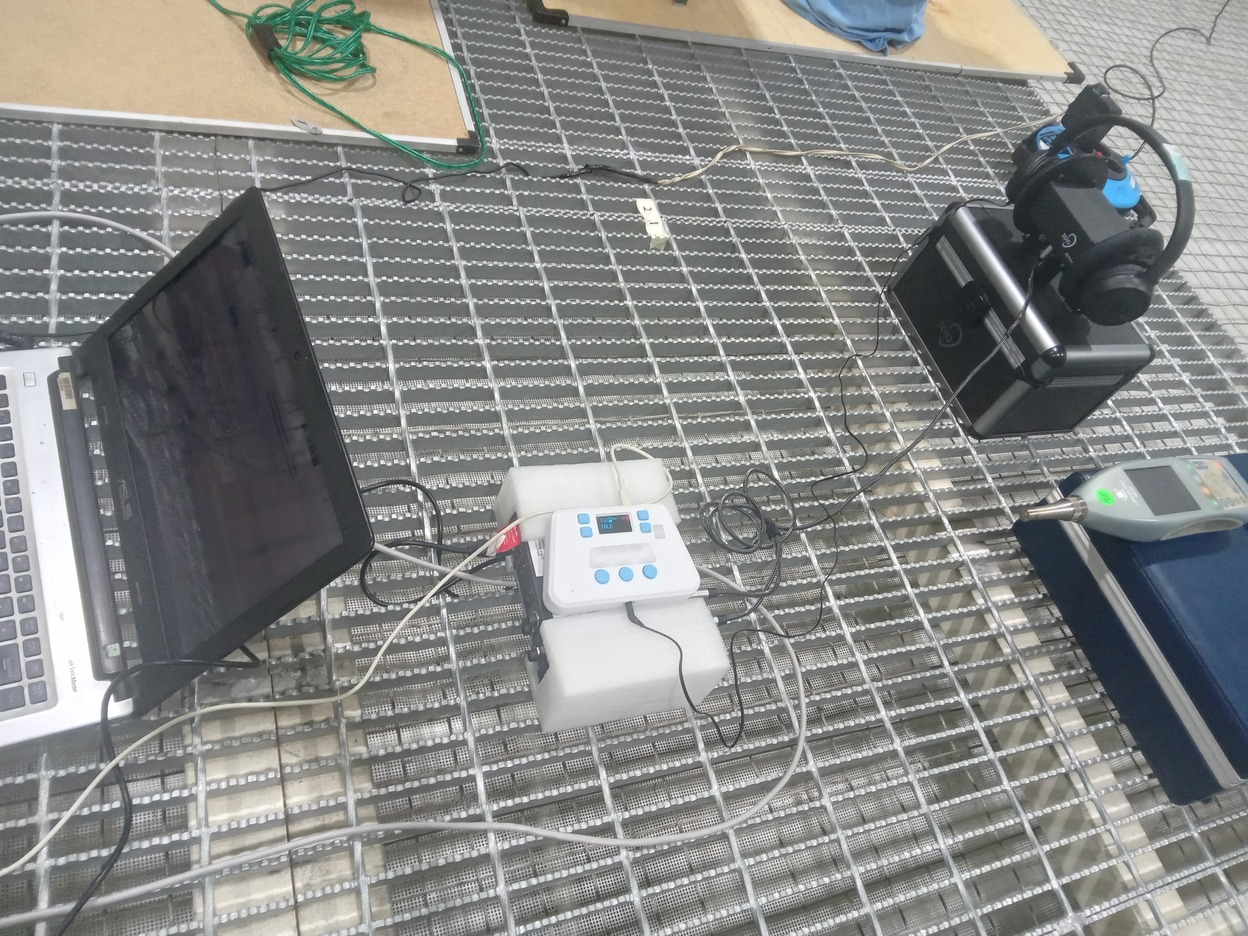
\includegraphics[width=\textwidth]{images/3dio_setup}
%			\caption{3DIO}
%		\end{subfigure}
%		\begin{subfigure}[]{.45\textwidth}
%			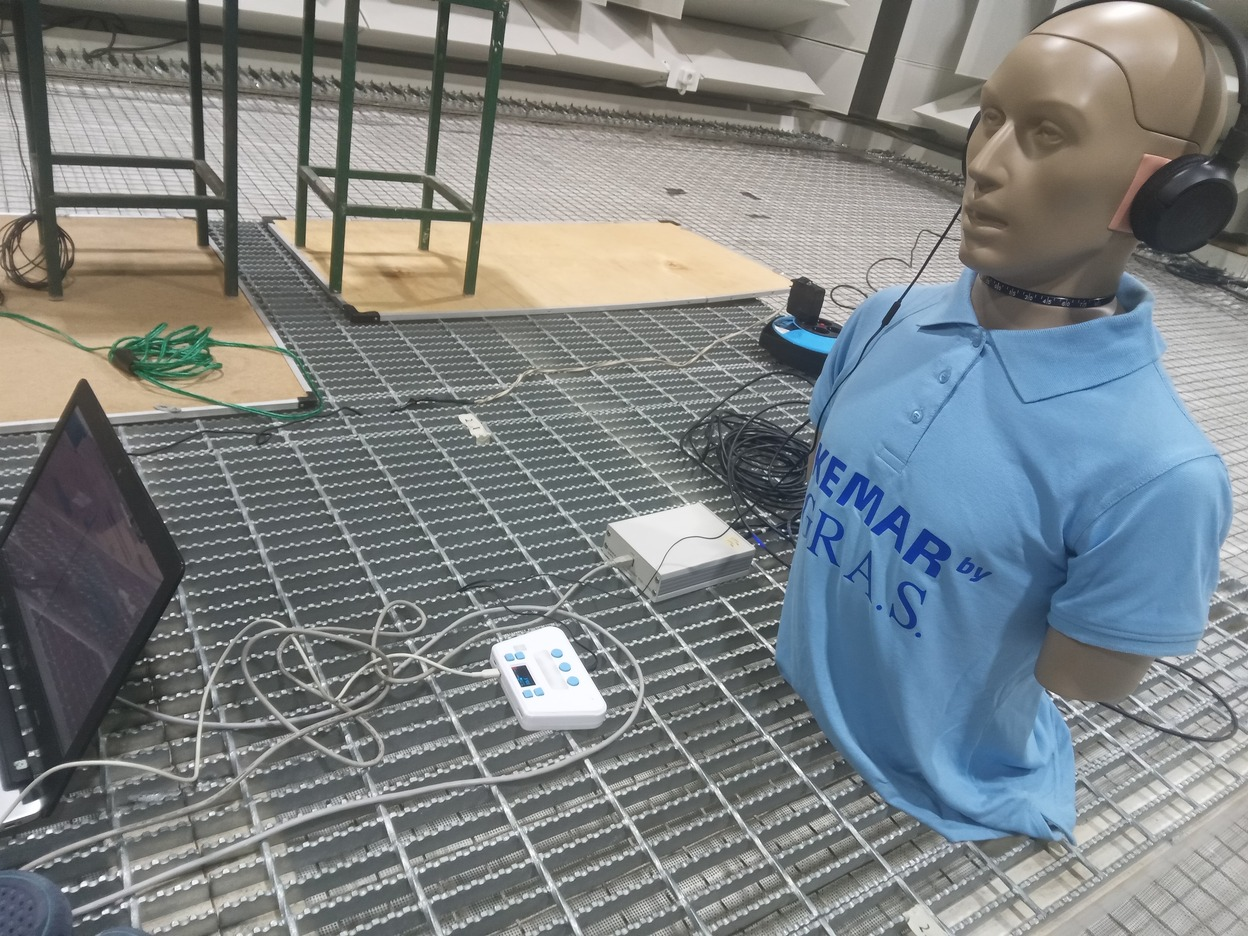
\includegraphics[width=\textwidth]{images/kemar_setup}
%			\caption{KEMAR}
%		\end{subfigure}
%		\\
%		\begin{subfigure}[]{.6\textwidth}
%			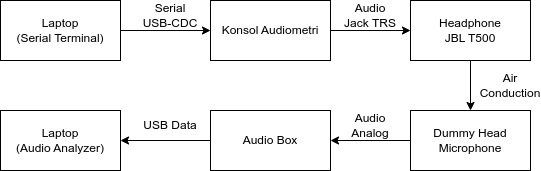
\includegraphics[width=\textwidth]{images/diagram/setup_uji}
%			\caption{Diagram}
%		\end{subfigure}
%		\caption{Setup Pengujian}
%	\end{figure}

	\begin{figure}[H]
		\centering
		\begin{subfigure}[]{.75\textwidth}
			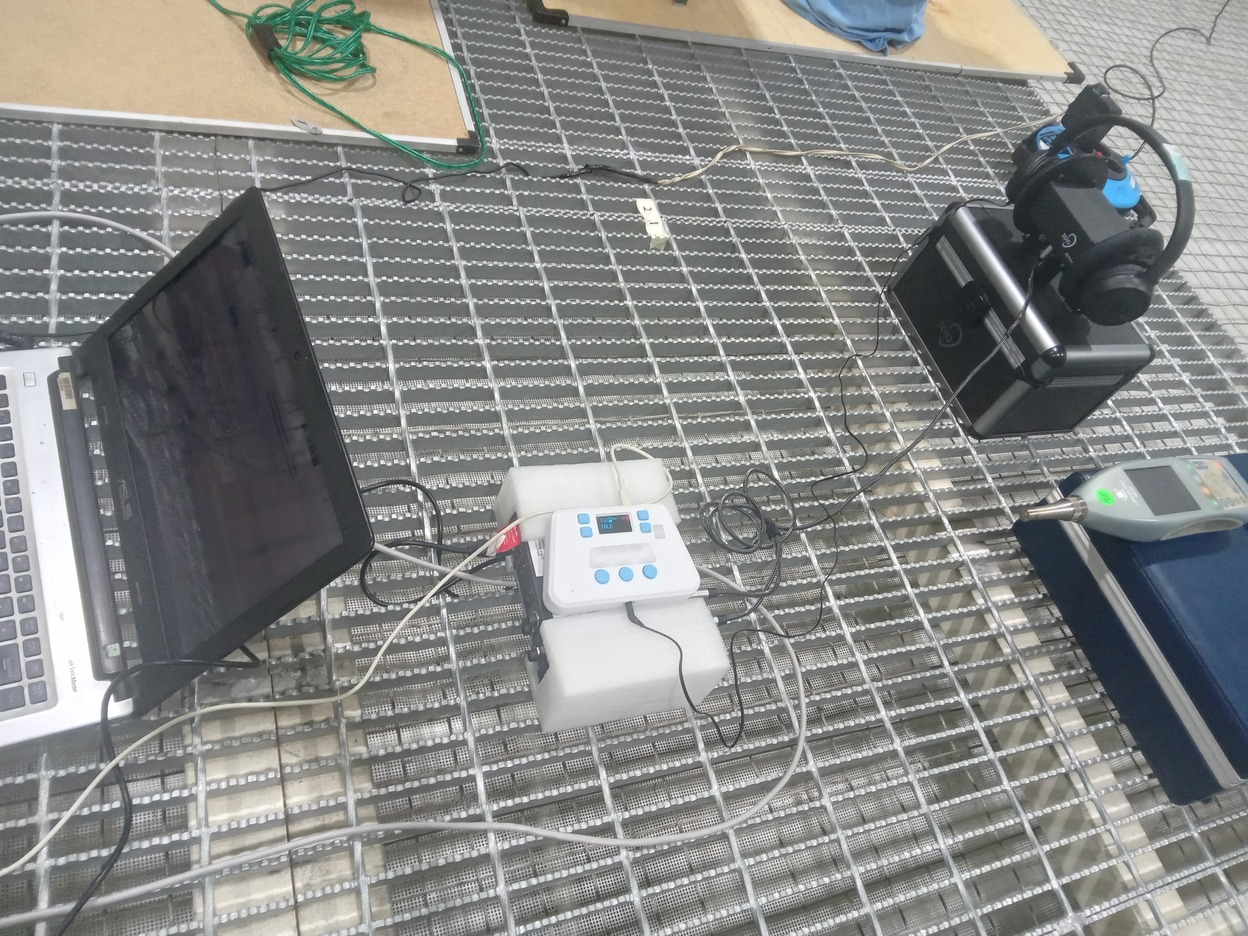
\includegraphics[width=\textwidth]{images/3dio_setup}
			\caption{3DIO}
		\end{subfigure}
		\\
		\begin{subfigure}[]{.75\textwidth}
			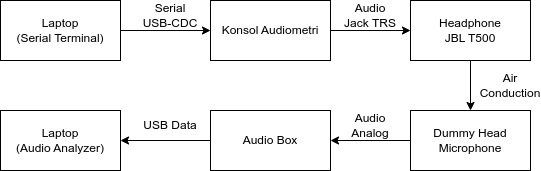
\includegraphics[width=\textwidth]{images/diagram/setup_uji}
			\caption{Diagram}
		\end{subfigure}
		\caption{Setup Pengujian}
	\end{figure}

	\newpage
	\subsection{Komunikasi Serial}

	\begin{enumerate}
		\item Berikut adalah perangkat lunak komunikasi serial ke Konsol yang perlu disiapkan untuk pengujian ini (panduan ini menggunakan Windows-7 32-bit sebagai contoh)

		\item Install driver ARM USB-CDC.\\
		Untuk dapat menghubungkan unit prototype dengan komputer,
		diperlukan driver ARM USB-CDC untuk komunikasi serial.

		\begin{itemize}
			\item File installer (sesuaikan dengan bit OS).
			Dapat didownload di \href{https://drive.google.com/drive/folders/19gXVrxR68SFHQUGGGgKb0Da03oV7Rh41?usp=share_link}{USB-CDC\_Driver}.
			\begin{figure}[H]
				\centering
				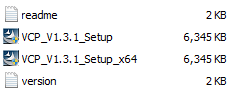
\includegraphics[width=200pt]{images/software/driver}
				\caption{Installer Driver}
			\end{figure}

			\item Instalasi driver (tanpa unit prototype terhubung) cukup mudah sebagaimana umumnya.
			\begin{figure}[H]
				\centering
				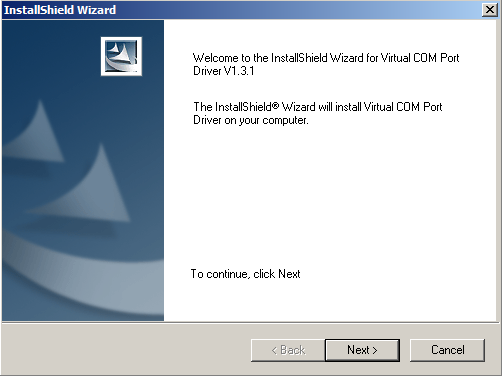
\includegraphics[width=200pt]{images/software/install_driver}
				\caption{Mulai instal driver}
			\end{figure}
		\end{itemize}

		\item Sambungkan unit prototype yang telah nyala dengan komputer via kabel USB.
		\begin{figure}[H]
			\centering
			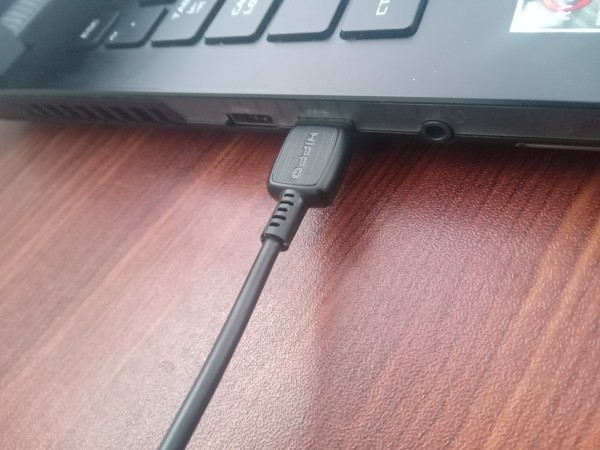
\includegraphics[width=200pt]{images/pasang/laptop_usb}
			\caption{Sambung Kabel USB ke Laptop}
		\end{figure}

		\item Tunggu hingga driver selesai mengkonfigurasi otomatis

		\item Cek \textit{Device Manager} untuk mengetahui Nomor Serial-Port
		\begin{itemize}
			\item Buka run-command dialog dengan kombinasi keyboard %(\keys{\WinKey + r})

			\item masukkan perintah \textbf{devmgmt.msc}.
			\begin{figure}[H]
				\centering
				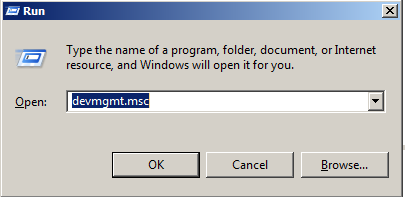
\includegraphics[width=200pt]{images/software/devicemgr}
				\caption{Memanggil Device Manager}
			\end{figure}

			\item Tekan (\keys{\return}) atau klik OK

			\item Cari entry \textit{Ports (COM and LPT)}.
			Catat nomor port untuk entry \textit{STMicroelectronics Virtual COM Port}.
			Dalam contoh ini, terkonfigurasi pada COM3.

			\begin{figure}[H]
				\centering
				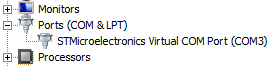
\includegraphics[width=200pt]{images/software/comport}
				\caption{Serial Komunikasi pada COM3}
			\end{figure}
		\end{itemize}


		\item Install Serial Terminal.
		Untuk dapat berkomunikasi via serial port, perlu diinstall serial terminal.
		Disini dicontohkan menggunakan \textit{Hercules}.

		\begin{itemize}
			\item Program terminal Hercules. Dapat didownload di \href{https://drive.google.com/drive/folders/1fgNPnGeSm20TrFfwmeCa4B24WIN_t_o_?usp=share_link}{Terminal}.
			\begin{figure}[H]
				\centering
				
\includegraphics[width=200pt]{images/software/hercules}
				\caption{Hercules Terminal}
			\end{figure}

			\item Jalankan program Hercules.
			Jika muncul konfirmasi lisensi, cukup \textit{Close} saja.

			\item Pilih tab \textit{Serial}.
			\begin{figure}[H]
				\centering
				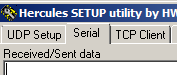
\includegraphics[width=200pt]{images/software/hercules_serial}
				\caption{Serial Terminal}
			\end{figure}
		\end{itemize}

		\item Test Komunikasi Serial
		\begin{itemize}
			\item Hercules Serial Terminal
			\begin{figure}[H]
				\centering
				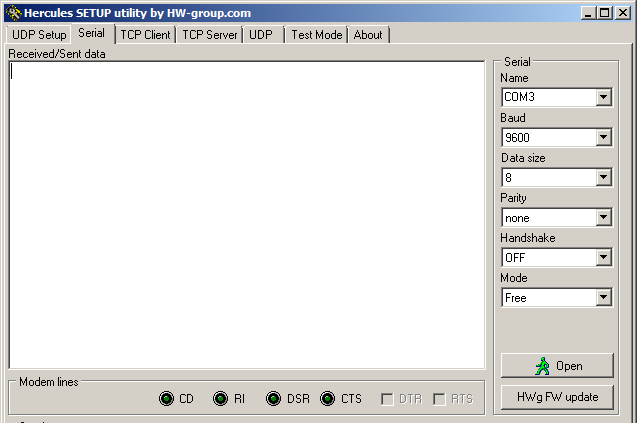
\includegraphics[width=250pt]{images/software/hercules_terminal}
				\caption{Hercules Serial Terminal}
			\end{figure}

			\item Setting Port pada Serial Terminal sebagai berikut
			\begin{itemize}
				\item Name     : COM3
				\item Baud     : 9600
				\item Data size: 8
				\item Parity   : none
			\end{itemize}

			\begin{figure}[H]
				\centering
				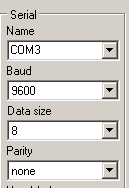
\includegraphics[width=100pt]{images/software/hercules_port}
				\caption{Pengaturan serial port}
			\end{figure}

			\item Klik Open (pastikan unit prototype sudah standby dan terhubung
			serta nama COM port sudah sesuai)

			\begin{figure}[H]
				\centering
				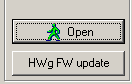
\includegraphics[width=100pt]{images/software/hercules_open}
				\caption{Open Serial Port}
			\end{figure}

			\item Kolom terminal akan menampilkan pesan:
			\begin{minted}[frame=lines,framesep=2mm,fontsize=\small]{text}
Serial port COM3 opened
			\end{minted}

			\item Selanjutnya, pada kolom terminal,
			masukkan perintah berikut dan diakhiri dengan (\keys{\return})
			\begin{minted}[frame=lines,framesep=2mm,fontsize=\small]{text}
info
			\end{minted}
			Serial akan menampilkan informasi kernel dan platform
			\begin{figure}[H]
				\centering
				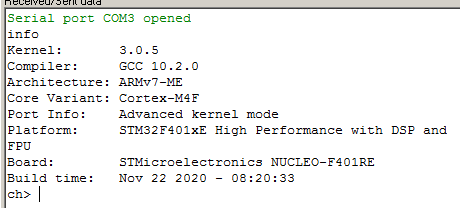
\includegraphics[width=300pt]{images/software/hercules_text}
				\caption{Informasi Platform}
			\end{figure}
		\end{itemize}

	\end{enumerate}

	Berikut beberapa contoh perintah serial yang dapat diakses melalui komunikasi serial Konsol:

	\begin{table}[H]
		\renewcommand{\tablename}{Tabel}
		\centering
		\caption{Contoh perintah serial yang tersedia pada konsol Audiometri.}
		\begin{tabular}{| p{0.05\textwidth} | p{0.1\textwidth} | p{0.15\textwidth} | p{0.2\textwidth} | p{0.4\textwidth} |}
			\hline
			\textbf{No} & \textbf{Perintah} & \textbf{Fungsi} & \textbf{Contoh Perintah} & \textbf{Contoh Respon} \\
			\hline
			1 & \textit{help} & Menampilkan Perintah yang tersedia & \textit{help} & \textit{coba mmc out tes led sig tone virt ...} \\
			\hline
			2 & \textit{info} & Menampilkan Info Platform Chip & \textit{info} & \textit{Kernel: 6.1.4Compiler: GCC 12.1.0 ...} \\
			\hline
			3 & \textit{mmc} & Mengelola isi SDCard & \textit{mmc} & \textit{usage: mmc [test|ls|lsnum| ...} \\
			& & & \textit{mmc ls} & \textit{HT1.TXT HT2.TXT ...} \\
			& & & \textit{mmc cat 1} & \textit{\{"audiogram":\{ ...} \\
			\hline
			4 & \textit{out} & Menghasilkan nada murni &  \textit{out} & \textit{usage: out <0/1> <freq> <ampl> ...} \\
			& & & \textit{out 500 11} & \textit{Out: Freq:  500 Ampl:11} \\
			& & & \textit{out 1 250 8} & \textit{Out: Freq:  250 Ampl:8} \\
			\hline
		\end{tabular}
	\end{table}

	\textbf{Keterangan}: Beberapa keterangan perintah \textit{out}:
	\begin{itemize}
		\item Pilihan Channel adalah 0 atau kosong untuk kiri, dan 1 untuk kanan.
		\item Pilihan Frekuensi Nada Murni: 125Hz, 250Hz, 500Hz, 1000Hz, 2000Hz, 4000Hz, dan 8000Hz.
		\item Pilihan Skala Loudness Nada Murni: 1, 2, 3, 4, 5, 6, 7, 8, 9, 10, dan 11.
	\end{itemize}

	\subsection{Kalibrasi Hearing Level Air Conduction}

	\begin{enumerate}
		\item Pengujian yang dimaksudkan untuk mendapatkan nilai aktual output audio nada murni dalam satuan dBA.

		\item Output nada murni memiliki karakteristik:
		\begin{itemize}
			\item frekuensi adalah nilai frekuensi (dalam Hz) yaitu 125, 250, 500, 1000, 2000, 4000, dan 8000.
			\item amplitudo adalah skala amplitudo antara 1 sampai 11.
		\end{itemize}

		\item Untuk perangkat lunak Audio Analyzer, digunakan program \textit{Real-Time Analyzer}
		yang merupakan bagian dari paket software DSFF3 buatan Yoshimasha.
		Jika membutuhkan versi trial dapat didownload di \url{http://intip.in/stm32tools}.

		Antar-muka Real-Time Analyzer yang digunakan adalah \textit{FFT-Analyzer} pada tab \textit{Octave band}.

		\begin{figure}[!ht]
			\centering
			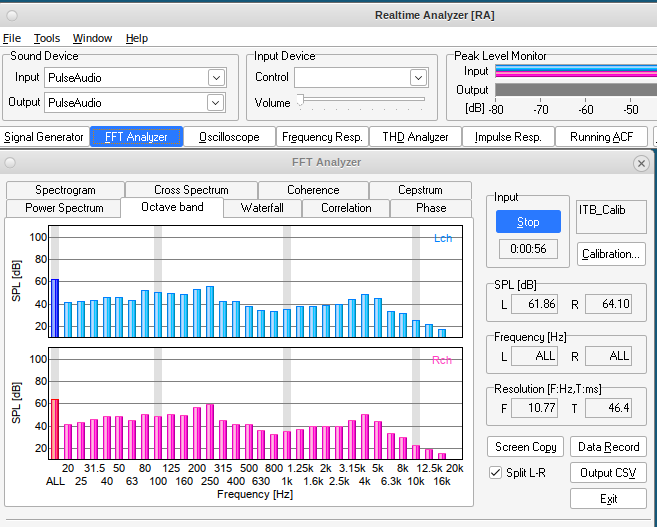
\includegraphics[width=0.45\textwidth]{images/rta_fft}
			\caption{Octave band pada FFT analyzer}
		\end{figure}

		Pada tampilan Octave-Band, klik satu bar frekuensi untuk mengetahui nilai SPL (dB)
		yang terisolasi dengan frekuensi lain.


		\item Berikut adalah prosedur untuk mencoba \textit{tone-generation}:
		\begin{enumerate}
			\item Nyalakan unit prototype dan tunggu standby.
			Pastikan USB belum terhubung ke komputer.
			\item Sambungkan unit dengan headphone yang disiapkan
			\item Sambungkan USB ke komputer
			\item Cek nomor COM port pada Device manager
			\item Jalankan Hercules terminal
			\item Atur nama port sesuai COM port
			\item Klik \textbf{Open} pada Hercules terminal
			\item Masukkan perintah berikut:
			\begin{minted}[frame=lines,framesep=2mm,fontsize=\small]{text}
				out 500 5
			\end{minted}
			\item Setelah tekan (\keys{\return}), maka pada salah satu headphone
			akan membangkitkan tone selama kurang lebih 5detik.
			\item Jika setelah selesai, tekan \textbf{Close} pada terminal,
			lepas USB, dan matikan unit prototype.

		\end{enumerate}

		\item Berikut contoh variasi perintah untuk menghasilkan nada murni (sebagaimana Tabel \ref{table:serial-code}):

		\begin{itemize}
			\item Nada murni pada frekuensi 500Hz dan skala 11.
			\begin{minted}[frame=lines,framesep=2mm,fontsize=\small]{text}
out 500 11
			\end{minted}

			\item Nada murni pada frekuensi 500Hz dan skala 1.
			\begin{minted}[frame=lines,framesep=2mm,fontsize=\small]{text}
out 500 1
			\end{minted}

			\item Nada murni pada frekuensi 500Hz dan skala 11 di channel/sisi kanan.
			\begin{minted}[frame=lines,framesep=2mm,fontsize=\small]{text}
out 1 500 11
			\end{minted}

			\textbf{Catatan:} Pengukuran dua sisi diperlukan jika diasumsikan headphone berbeda karakteristik kedua sisinya.
		\end{itemize}

		\begin{table}[H]
			\renewcommand{\tablename}{Tabel}
			\caption{Format tabel hasil uji nada murni dalam dB-SPL}
			\centering
			\begin{tabular}{|p{0.07\linewidth}|c|c|c|c|c|c|c|c|c|c|c|}
				\hline
				Scale/ Freq & 11 & 10 & 9 & 8 & 7 & 6 & 5 & 4 & 3 & 2 & 1\\ [0.5ex]
				\hline\hline
				125Hz & x  & x  & x  & x  & x  & x  & x  & x  & x  & x  & x \\
				\hline
				250Hz & x  & x  & x  & x  & x  & x  & x  & x  & x  & x  & x \\
				\hline
				500Hz & x  & x  & x  & x  & x  & x  & x  & x  & x  & x  & x \\
				\hline
				1000Hz & x  & x  & x  & x  & x  & x  & x  & x  & x  & x  & x \\
				\hline
				2000Hz & x  & x  & x  & x  & x  & x  & x  & x  & x  & x  & x \\
				\hline
				4000Hz & x  & x  & x  & x  & x  & x  & x  & x  & x  & x  & x \\
				\hline
				8000Hz & x  & x  & x  & x  & x  & x  & x  & x  & x  & x  & x \\
				\hline
			\end{tabular}
		\end{table}
	\end{enumerate}

	\newpage
	\section{Hasil Pengujian}

	\subsection{Unduh Data}

	Kumpulan data dalam format tabel CSV dapat diunduh dalam repository Github berikut:
	\url{https://github.com/VibrasticLab/pikoakustik2/tree/master/prototrial/dokumen/berita_acara/itb_july2023/data_records}\\

	Skrip Python untuk ekstraksi data dapat dilihat di:
	\url{https://github.com/VibrasticLab/pikoakustik2/blob/master/prototrial/dokumen/berita_acara/itb_july2023/data_records/extract_table.py}

	\subsection{Tabel Hasil}

	Berikut hasil pengukuran dalam bentuk tabel untuk satuan dB-SPL:

	\subsubsection{Hasil dari 3DIO}

	\begin{table}[H]
		\renewcommand{\tablename}{Tabel}
		\caption{Tabel hasil uji nada murni dalam dB-SPL untuk channel Kiri}
		\centering
		\begin{tabular}{|p{0.07\linewidth}|c|c|c|c|c|c|c|c|c|c|c|}
			\hline
			Scale/ Freq & 11 & 10 & 9 & 8 & 7 & 6 & 5 & 4 & 3 & 2 & 1\\ [0.5ex]
			\hline\hline
			125Hz & 62.3 & 56.3 & 50.3  & 44.2 & 38.1 & 31.8 & 25.1 & 17.8 & 9.9 & -2.9 & -2 \\
			250Hz & 63.9 & 57.9 & 51.8  & 45.7 & 39.6 & 33.3 & 26.7 & 19.6 & 12.3 & -5.9 & -6 \\
			500Hz & 67.0 & 60.9 & 54.9  & 48.8 & 42.6 & 36.4 & 29.8 & 22.4 & 14.8 & -6.0 & -5 \\
			1000Hz & 76.9 & 70.9 & 64.8  & 58.7 & 52.6 & 46.3 & 39.8 & 32.6 & 24.7 & -2.9 & -4 \\
			2000Hz & 71.3 & 65.2 & 59.2  & 53.1 & 47.0 & 40.7 & 34.2 & 26.9 & 19.1 & -4.2 & -4 \\
			4000Hz & 79.2 & 73.1 & 67.1  & 61.0 & 54.9 & 48.6 & 42.0 & 34.5 & 26.4 & 2.1 & 2 \\
			8000Hz & 87.5 & 81.4 & 75.3  & 69.3 & 63.1 & 56.8 & 50.5 & 43.8 & 36.4 & 12.0 & 11 \\
			\hline
		\end{tabular}
	\end{table}

	\begin{table}[H]
		\renewcommand{\tablename}{Tabel}
		\caption{Tabel hasil uji nada murni dalam dB-SPL untuk channel Kanan}
		\centering
		\begin{tabular}{|p{0.07\linewidth}|c|c|c|c|c|c|c|c|c|c|c|}
			\hline
			Scale/ Freq & 11 & 10 & 9 & 8 & 7 & 6 & 5 & 4 & 3 & 2 & 1\\ [0.5ex]
			\hline\hline
			125Hz & 64.6 & 58.6 & 52.6  & 46.5 & 40.3 & 34.1 & 27.5 & 20.2 & 12.4 & 0.4 & -1 \\
			250Hz & 66.2 & 60.1 & 54.1  & 48.0 & 41.8 & 35.6 & 28.9 & 21.7 & 13.9 & -5.0 & -4 \\
			500Hz & 68.7 & 62.7 & 56.6  & 50.6 & 44.4 & 38.1 & 31.5 & 24.3 & 16.6 & -4.7 & -5 \\
			1000Hz & 76.9 & 70.9 & 64.8  & 58.7 & 52.6 & 46.3 & 39.8 & 32.5 & 24.7 & -2.4 & -4 \\
			2000Hz & 69.5 & 63.5 & 57.4  & 51.3 & 45.2 & 38.9 & 32.4 & 25.2 & 17.3 & -5.3 & -4 \\
			4000Hz & 79.7 & 73.6 & 67.6  & 61.5 & 55.4 & 49.1 & 42.5 & 35.0 & 26.9 & 1.3 & 2 \\
			8000Hz & 86.6 & 80.6 & 74.5  & 68.4 & 62.3 & 56.0 & 49.7 & 43.0 & 35.6 & 11.5 & 12 \\
			\hline
		\end{tabular}
	\end{table}

%	\subsubsection{Hasil dari KEMAR}
%
%	\begin{table}[H]
%		\renewcommand{\tablename}{Tabel}
%		\caption{Tabel hasil uji nada murni dalam dB-SPL untuk channel Kiri}
%		\centering
%		\begin{tabular}{|p{0.07\linewidth}|c|c|c|c|c|c|c|c|c|c|c|}
%			\hline
%			Scale/ Freq & 11 & 10 & 9 & 8 & 7 & 6 & 5 & 4 & 3 & 2 & 1\\ [0.5ex]
%			\hline\hline
%			125Hz & 58.40 & 52.40 & 46.35  & 40.25 & 34.06 & 27.74 & 21.35 & 14.52 & 9.45 & 3.42 & 6 \\
%			250Hz & 58.15 & 52.12 & 46.06  & 39.94 & 33.78 & 27.57 & 21.45 & 13.95 & 7.84 & 1.94 & 1 \\
%			500Hz & 59.76 & 53.72 & 47.64  & 41.56 & 35.45 & 29.20 & 22.39 & 15.58 & 8.02 & 1.38 & 1 \\
%			1000Hz & 65.97 & 59.93 & 53.87  & 47.77 & 41.59 & 35.32 & 28.77 & 21.44 & 13.18 & 0.58 & 1 \\
%			2000Hz & 59.79 & 53.74 & 47.69  & 41.60 & 35.47 & 29.16 & 22.74 & 15.06 & 9.05 & 2.84 & 3 \\
%			4000Hz & 69.54 & 63.50 & 57.46  & 51.38 & 45.26 & 38.97 & 32.37 & 24.85 & 17.06 & 6.75 & 6 \\
%			8000Hz & 71.50 & 65.45 & 59.36  & 53.31 & 47.15 & 40.91 & 34.63 & 27.98 & 20.81 & 9.06 & 9 \\
%			\hline
%		\end{tabular}
%	\end{table}
%
%	\begin{table}[H]
%		\renewcommand{\tablename}{Tabel}
%		\caption{Tabel hasil uji nada murni dalam dB-SPL untuk channel Kanan}
%		\centering
%		\begin{tabular}{|p{0.07\linewidth}|c|c|c|c|c|c|c|c|c|c|c|}
%			\hline
%			Scale/ Freq & 11 & 10 & 9 & 8 & 7 & 6 & 5 & 4 & 3 & 2 & 1\\ [0.5ex]
%			\hline\hline
%			125Hz & 53.24 & 47.25 & 41.16  & 35.18 & 28.91 & 22.71 & 15.65 & 9.51 & 4.43 & 5.63 & 2 \\
%			250Hz & 53.30 & 47.25 & 41.19  & 35.16 & 28.87 & 22.88 & 16.01 & 10.07 & 4.14 & 1.92 & 0 \\
%			500Hz & 57.07 & 51.00 & 44.95  & 38.89 & 32.73 & 26.54 & 19.89 & 13.02 & 6.96 & -1.30 & -1 \\
%			1000Hz & 64.97 & 58.93 & 52.87  & 46.80 & 40.65 & 34.38 & 27.86 & 20.70 & 13.08 & -2.07 & -2 \\
%			2000Hz & 59.03 & 52.99 & 46.93  & 40.83 & 34.66 & 28.40 & 21.98 & 14.74 & 7.96 & 0.09 & -1 \\
%			4000Hz & 78.40 & 72.37 & 66.33  & 60.23 & 54.12 & 47.83 & 41.26 & 33.70 & 25.64 & 3.51 & 4 \\
%			8000Hz & 64.56 & 58.51 & 52.42  & 46.39 & 40.22 & 33.98 & 27.68 & 21.18 & 13.89 & 5.14 & 5 \\
%			\hline
%		\end{tabular}
%	\end{table}

\end{document}
